
\documentclass[10pt]{article}

\usepackage[a4paper,margin=0.65in]{geometry}
\usepackage{amsmath,amssymb}
\usepackage{graphicx}
\usepackage{booktabs}
\usepackage{array}
\usepackage{float}
\usepackage{hyperref}
\usepackage{enumitem}
\usepackage{xcolor}
\usepackage{tikz}
\usetikzlibrary{positioning,arrows.meta,shapes.geometric,fit,calc}

\setlist{nosep,leftmargin=*}
\renewcommand{\arraystretch}{1.2}
\setlength{\parindent}{0pt}
\setlength{\parskip}{2pt}

% Placeholder box for plots -- to be replaced with \includegraphics once
% the corresponding figure is exported from the notebook and uploaded here.
\newcommand{\plotplaceholder}[1]{%
\begin{center}
\fbox{\parbox[c][5cm]{0.85\textwidth}{\centering
\vspace{1cm}
\textit{[Insert #1 here]}\\[0.3cm]
\footnotesize (Export the corresponding figure from the notebook and replace this box with\\
\texttt{\textbackslash includegraphics[width=0.85\textwidth]\{...\}})
\vspace{1cm}
}}
\end{center}
}

% Blank answer space for discussion questions.
\newcommand{\answerspace}{\vspace{0.2cm}\textit{Answer:}\\[1.6cm]}

\tikzset{
layer/.style={
draw,
rounded corners,
minimum width=1.7cm,
minimum height=0.65cm,
align=center,
fill=blue!10,
font=\scriptsize
},
smalllayer/.style={
draw,
rounded corners,
minimum width=1.35cm,
minimum height=0.58cm,
align=center,
fill=green!10,
font=\scriptsize
},
arrow/.style={
-{Latex[length=2mm]},
thin
}
}

\begin{document}

%%%%%%%%%%%%%%%%%%%%%%%%%%%%%%%%%%%%%%%%%%%%%%%%%%%%%%%%%%%%
% TITLE
%%%%%%%%%%%%%%%%%%%%%%%%%%%%%%%%%%%%%%%%%%%%%%%%%%%%%%%%%%%%

\begin{center}

{\large\textbf{Shiv Nadar University Chennai}}

\vspace{2mm}

{\normalsize\textbf{CS3807 -- Deep Learning Laboratory}}

\vspace{2mm}

{\large\textbf{Experiment 6}}

\vspace{1mm}

{\normalsize\textbf{End-to-End Study of RNN, LSTM and GRU for}}

{\normalsize\textbf{Sequence Learning and Video Understanding}}

\end{center}

\vspace{3mm}

\begin{tabular}{|p{3.4cm}|p{9.0cm}|p{1.4cm}|}
\hline
Degree \& Branch &
B.Tech Artificial Intelligence \& Data Science &
Semester V\\
\hline
Subject Code \& Name &
CS3807 -- Deep Learning Laboratory &
AY: 2026--27\\
\hline
\end{tabular}\\ \\
\url{https://github.com/atishmandal/CS3807-Deep-Learning-Lab/tree/main/lab6}
%%%%%%%%%%%%%%%%%%%%%%%%%%%%%%%%%%%%%%%%%%%%%%%%%%%%%%%%%%%%
\section*{1. Objective}

The objective of this experiment is to develop an end-to-end understanding of
recurrent sequence learning by implementing and comparing Vanilla RNN, LSTM
and GRU models. The experiment also introduces Backpropagation Through Time
(BPTT), the limitations of conventional RNNs, and the use of CNN-extracted
features with recurrent networks for video understanding.

The experiment uses the UCI Human Activity Recognition Using Smartphones
dataset as the primary sequence dataset. Students will prepare temporal input
sequences, visualize them, train RNN/LSTM/GRU models, compare their
performance, analyze convergence and generalization, and extend the pipeline
to video understanding using CNN feature extraction followed by an LSTM or
GRU.

A small synthetic sequence-to-sequence task is included at the end to
demonstrate the encoder--decoder framework.

%%%%%%%%%%%%%%%%%%%%%%%%%%%%%%%%%%%%%%%%%%%%%%%%%%%%%%%%%%%%
\section*{2. Learning Outcomes}

After completing this experiment, students will be able to:

\begin{itemize}
\item represent sequential data using the $(N,T,F)$ input format;
\item explain the architecture and operation of a Vanilla RNN;
\item explain Backpropagation Through Time and the vanishing/exploding gradient challenges;
\item implement sequence classification using SimpleRNN, LSTM and GRU;
\item compare RNN, LSTM and GRU using quantitative performance measures;
\item interpret training/validation curves and confusion matrices;
\item explain the role of CNNs in extracting spatial features from video frames;
\item construct a CNN--LSTM or CNN--GRU pipeline for video understanding;
\item explain the encoder--decoder architecture for sequence-to-sequence learning; and
\item draw conclusions using predictive performance, model complexity and computational cost.
\end{itemize}

%%%%%%%%%%%%%%%%%%%%%%%%%%%%%%%%%%%%%%%%%%%%%%%%%%%%%%%%%%%%
\section*{3. Dataset and Experimental Setup}

\textbf{Primary Dataset: UCI Human Activity Recognition Using Smartphones}

The UCI Human Activity Recognition (HAR) dataset contains smartphone sensor
measurements collected from subjects performing six activities:

\begin{itemize}
\item WALKING
\item WALKING\_UPSTAIRS
\item WALKING\_DOWNSTAIRS
\item SITTING
\item STANDING
\item LAYING
\end{itemize}

The experiment should use the raw inertial signal files rather than only the
already-computed 561-feature vectors. Each activity window contains 128
temporal measurements. The three-axis body acceleration, three-axis
gyroscope and three-axis total acceleration signals provide nine channels.

Thus, the desired input representation is

\[
X\in\mathbb{R}^{N\times128\times9}.
\]

The dataset can be obtained from:

\url{https://archive.ics.uci.edu/dataset/240/human+activity+recognition+using+smartphones}

\textbf{Recommended laboratory subset:} To keep execution time small, use
the first 1500--3000 training windows while preserving all six classes and
approximately balanced class representation. For a complete study, the full
training and test partitions may be used.

\textbf{Important:} The same train/validation/test protocol and preprocessing
must be used for RNN, LSTM and GRU so that the comparison is controlled.

\subsection*{Expected Input}

For one sample:

\[
X_i\in\mathbb{R}^{128\times9}.
\]

For a batch of 32 samples:

\[
X_{\mathrm{batch}}\in\mathbb{R}^{32\times128\times9}.
\]

The dimensions represent:

\begin{center}
\begin{tabular}{|c|c|l|}
\hline
Dimension & Meaning & Example\\
\hline
$N$ & Number of sequences & 1500\\
$T$ & Time steps per sequence & 128\\
$F$ & Features/channels per time step & 9\\
\hline
\end{tabular}
\end{center}

Therefore, the model must receive a three-dimensional tensor rather than a
conventional two-dimensional tabular matrix.

%%%%%%%%%%%%%%%%%%%%%%%%%%%%%%%%%%%%%%%%%%%%%%%%%%%%%%%%%%%%
\section*{4. Overall Experimental Pipeline}

The complete sequence-classification pipeline is:

\begin{center}
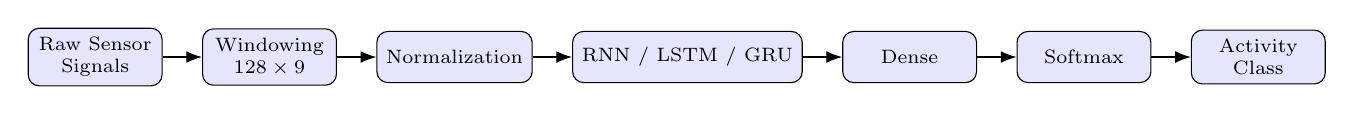
\begin{tikzpicture}[node distance=5mm]
\node[layer](a){Raw Sensor\\Signals};
\node[layer,right=of a](b){Windowing\\$128\times9$};
\node[layer,right=of b](c){Normalization};
\node[layer,right=of c](d){RNN / LSTM / GRU};
\node[layer,right=of d](e){Dense};
\node[layer,right=of e](f){Softmax};
\node[layer,right=of f](g){Activity\\Class};

\foreach \x/\y in {a/b,b/c,c/d,d/e,e/f,f/g}
\draw[arrow](\x)--(\y);
\end{tikzpicture}
\end{center}

The three recurrent models must use the same input, output layer, optimizer,
batch size and evaluation protocol.

%%%%%%%%%%%%%%%%%%%%%%%%%%%%%%%%%%%%%%%%%%%%%%%%%%%%%%%%%%%%
\section*{5. Preprocessing}

Perform the following preprocessing steps:

\begin{enumerate}
\item Load the raw inertial signals.
\item Arrange every observation window as $128\times9$.
\item Assign one activity label to each window.
\item Encode the six activity labels.
\item Normalize the input using statistics calculated from the training data.
\item Create training, validation and test sets.
\item Verify the class distribution.
\end{enumerate}

\textbf{Suggested split:}

\[
70\% \text{ training},\qquad
15\% \text{ validation},\qquad
15\% \text{ testing}.
\]

The test data must not be used during model selection or hyperparameter tuning.

\subsection*{Expected Preprocessing Output}

Students must print:

\begin{verbatim}
Input tensor shape:
Training   : (2100, 128, 9)
Validation : (450,  128, 9)
Testing    : (450,  128, 9)

Number of classes: 6
Number of features per time step: 9
Sequence length: 128
\end{verbatim}

A class-balanced subset of 3000 windows (500 per activity) was drawn from
the official training partition and then split 70/15/15, giving
$N_{\mathrm{train}}=2100$, $N_{\mathrm{val}}=450$ and $N_{\mathrm{test}}=450$,
with the class distribution kept exactly balanced in every split
(350/75/75 windows per class in train/validation/test respectively).

%%%%%%%%%%%%%%%%%%%%%%%%%%%%%%%%%%%%%%%%%%%%%%%%%%%%%%%%%%%%
\section*{6. Temporal Data Visualization}

Select representative sequences from at least three different activity
classes.

\textbf{Plot 1: Sensor signal versus time}

\begin{itemize}
\item X-axis: Time step (1--128)
\item Y-axis: Sensor value
\item Plot at least three representative channels.
\item Include examples from different activity classes.
\end{itemize}

\begin{figure}[H]
    \centering
    \includegraphics[width=0.85\textwidth]{Sensorvstime.png}
    \caption{Sensor signal vs. time for walking, walking downstairs, and laying.}
    \label{fig:sensor-signal}
\end{figure}

Students should observe that temporal patterns differ across activities.

\textbf{Required inference:}

\begin{enumerate}
\item \textbf{What temporal pattern is visible?} The dynamic activities (WALKING,
WALKING\_DOWNSTAIRS) show clearly periodic, high-amplitude oscillations in
reflecting the repeating cycle. LAYING shows a near-flat, low-variance
signal with a roughly constant offset (the \texttt{total\_acc\_x} channel
sits close to -1.6g, and almost
no gyroscope activity.
\item \textbf{Which activities exhibit similar patterns?} WALKING and
WALKING\_DOWNSTAIRS both show periodic oscillatory behaviour with comparable
frequency. However WALKING\_DOWNSTAIRS has larger amplitude spikes (from
impact on each step). LAYING is visually similar to the other static
activities (SITTING, STANDING). All three are dominated by the
constant gravity component rather than oscillation.
\item \textbf{Why is the ordering of measurements important?} The recurrent
model relies on the temporal ordering of the 128 samples to infer motion. Shuffling the time steps
within a window would destroy the sequence.
\end{enumerate}

%%%%%%%%%%%%%%%%%%%%%%%%%%%%%%%%%%%%%%%%%%%%%%%%%%%%%%%%%%%%
\section*{7. Vanilla RNN Architecture}

A Vanilla RNN maintains a hidden state that is updated at every time step:

\[
h_t=\tanh(W_xx_t+W_hh_{t-1}+b_h).
\]

The output can be written as

\[
y_t=g(W_yh_t+b_y).
\]

For sequence classification, the final hidden representation can be passed
to a classifier.

\begin{center}
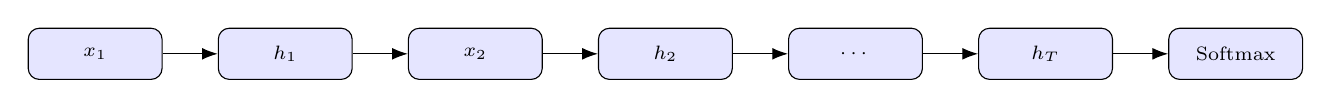
\begin{tikzpicture}[node distance=7mm]
\node[layer](x1){$x_1$};
\node[layer,right=of x1](h1){$h_1$};
\node[layer,right=of h1](x2){$x_2$};
\node[layer,right=of x2](h2){$h_2$};
\node[layer,right=of h2](x3){$\cdots$};
\node[layer,right=of x3](h3){$h_T$};
\node[layer,right=of h3](y){Softmax};

\draw[arrow](x1)--(h1);
\draw[arrow](h1)--(x2);
\draw[arrow](x2)--(h2);
\draw[arrow](h2)--(x3);
\draw[arrow](x3)--(h3);
\draw[arrow](h3)--(y);
\end{tikzpicture}
\end{center}

The diagram represents the unrolled view of an RNN. The same recurrent weights
are reused across time steps.

%%%%%%%%%%%%%%%%%%%%%%%%%%%%%%%%%%%%%%%%%%%%%%%%%%%%%%%%%%%%
\section*{8. Backpropagation Through Time}

When an RNN is unrolled, the loss depends on the sequence of hidden states.
Backpropagation Through Time (BPTT) propagates the error backward through
the recurrent steps.

\begin{center}
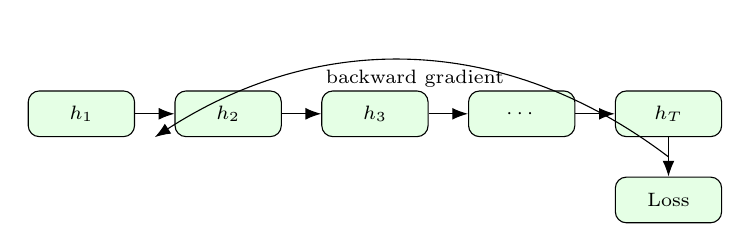
\begin{tikzpicture}[node distance=5mm]
\node[smalllayer](a){$h_1$};
\node[smalllayer,right=of a](b){$h_2$};
\node[smalllayer,right=of b](c){$h_3$};
\node[smalllayer,right=of c](d){$\cdots$};
\node[smalllayer,right=of d](e){$h_T$};
\node[smalllayer,below=of e](l){Loss};

\draw[arrow](a)--(b);
\draw[arrow](b)--(c);
\draw[arrow](c)--(d);
\draw[arrow](d)--(e);
\draw[arrow](e)--(l);

\draw[arrow]($(e.south)!0.5!(l.north)$) to[bend right=35]
node[below,font=\scriptsize]{backward gradient} ($(a.south)!0.5!(b.south)$);
\end{tikzpicture}
\end{center}

Students should explain that repeated multiplication of derivatives through
many time steps can cause gradients to become extremely small or extremely
large.

\subsection*{Challenges}

\begin{itemize}
\item Vanishing gradients
\item Exploding gradients
\item Difficulty learning long-term dependencies
\item Sequential computation and limited parallelism
\end{itemize}

The vanishing-gradient problem can be conceptually represented as

\[
\left|\frac{\partial h_t}{\partial h_{t-k}}\right|\rightarrow0
\]

while exploding gradients correspond to very large gradient magnitudes.

\subsection*{Numerical Exercise}

Consider

\[
x_1=0.5,\qquad x_2=0.7,\qquad x_3=0.2,
\]

\[
h_0=0,\qquad W_x=0.5,\qquad W_h=0.8,\qquad b=0.1.
\]

Using

\[
h_t=\tanh(W_xx_t+W_hh_{t-1}+b),
\]

calculate $h_1$, $h_2$ and $h_3$ manually.

Students must compare their calculated values with the values obtained from
a program.

\textbf{Computed values (manual recurrence, verified against a 1-unit
\texttt{SimpleRNNCell} initialised with the same weights):}

\[
h_1 = 0.336376,\qquad h_2 = 0.616352,\qquad h_3 = 0.599958.
\]

The manually computed values matched the Keras \texttt{SimpleRNNCell} output
exactly (\texttt{Keras } $h_1=0.336376$, $h_2=0.616352$, $h_3=0.599958$),
confirming the correctness of the recurrence implementation.

%%%%%%%%%%%%%%%%%%%%%%%%%%%%%%%%%%%%%%%%%%%%%%%%%%%%%%%%%%%%
\section*{9. RNN Implementation}

Use a small recurrent architecture:

\begin{center}
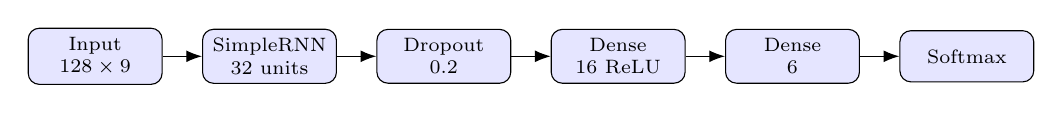
\begin{tikzpicture}[node distance=5mm]
\node[layer](a){Input\\$128\times9$};
\node[layer,right=of a](b){SimpleRNN\\32 units};
\node[layer,right=of b](c){Dropout\\0.2};
\node[layer,right=of c](d){Dense\\16 ReLU};
\node[layer,right=of d](e){Dense\\6};
\node[layer,right=of e](f){Softmax};

\foreach \x/\y in {a/b,b/c,c/d,d/e,e/f}
\draw[arrow](\x)--(\y);
\end{tikzpicture}
\end{center}

\textbf{Suggested training configuration:}

\begin{center}
\begin{tabular}{|l|l|}
\hline
Parameter & Value\\
\hline
Recurrent units & 32\\
Dropout & 0.2\\
Optimizer & Adam\\
Learning rate & $10^{-3}$\\
Batch size & 32\\
Epochs & 30\\
Loss & Sparse categorical cross-entropy\\
\hline
\end{tabular}
\end{center}

%%%%%%%%%%%%%%%%%%%%%%%%%%%%%%%%%%%%%%%%%%%%%%%%%%%%%%%%%%%%
\section*{10. LSTM Architecture}

LSTM introduces a memory cell and gates to control information flow.

The forget gate is

\[
f_t=\sigma(W_f[h_{t-1},x_t]+b_f),
\]

the input gate is

\[
i_t=\sigma(W_i[h_{t-1},x_t]+b_i),
\]

and the output gate is

\[
o_t=\sigma(W_o[h_{t-1},x_t]+b_o).
\]

The candidate cell state is

\[
\tilde{C}_t=
\tanh(W_C[h_{t-1},x_t]+b_C),
\]

and the cell state is

\[
C_t=f_tC_{t-1}+i_t\tilde{C}_t.
\]

The hidden state is

\[
h_t=o_t\tanh(C_t).
\]

\begin{center}
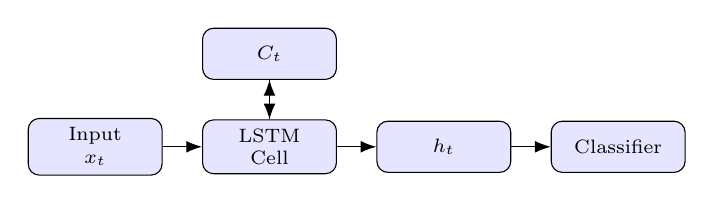
\begin{tikzpicture}[node distance=5mm]
\node[layer](a){Input\\$x_t$};
\node[layer,right=of a](b){LSTM\\Cell};
\node[layer,right=of b](c){$h_t$};
\node[layer,above=of b](d){$C_t$};
\node[layer,right=of c](e){Classifier};

\draw[arrow](a)--(b);
\draw[arrow](b)--(c);
\draw[arrow](b)--(d);
\draw[arrow](c)--(e);
\draw[arrow](d)--(b);
\end{tikzpicture}
\end{center}

\textbf{Required inference:} Explain how the cell state and gates help the
network retain or discard information over long sequences.

%%%%%%%%%%%%%%%%%%%%%%%%%%%%%%%%%%%%%%%%%%%%%%%%%%%%%%%%%%%%
\section*{11. GRU Architecture}

GRU uses two principal gates:

\[
z_t=\sigma(W_z[h_{t-1},x_t]+b_z)
\]

and

\[
r_t=\sigma(W_r[h_{t-1},x_t]+b_r).
\]

The candidate hidden state is

\[
\tilde{h}_t=
\tanh(W_h[r_t\odot h_{t-1},x_t]+b_h).
\]

The hidden state is updated using

\[
h_t=(1-z_t)h_{t-1}+z_t\tilde{h}_t.
\]

\begin{center}
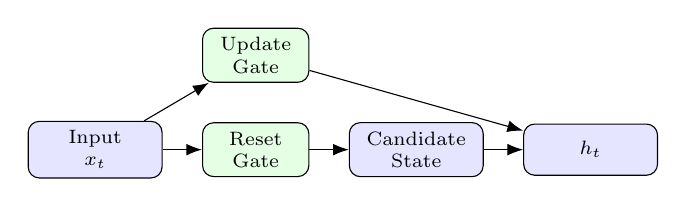
\begin{tikzpicture}[node distance=5mm]
\node[layer](a){Input\\$x_t$};
\node[smalllayer,right=of a](b){Reset\\Gate};
\node[smalllayer,above=of b](c){Update\\Gate};
\node[layer,right=of b](d){Candidate\\State};
\node[layer,right=of d](e){$h_t$};

\draw[arrow](a)--(b);
\draw[arrow](a)--(c);
\draw[arrow](b)--(d);
\draw[arrow](c)--(e);
\draw[arrow](d)--(e);
\end{tikzpicture}
\end{center}

Students should compare the number of gates and state representations in
RNN, LSTM and GRU.

%%%%%%%%%%%%%%%%%%%%%%%%%%%%%%%%%%%%%%%%%%%%%%%%%%%%%%%%%%%%
\section*{12. LSTM and GRU Implementation}

Implement the same classifier used for the RNN, replacing only the recurrent
layer.

\begin{center}
\begin{tabular}{|l|c|c|c|}
\hline
Model & Recurrent Layer & Units & Output Classes\\
\hline
RNN & SimpleRNN & 32 & 6\\
LSTM & LSTM & 32 & 6\\
GRU & GRU & 32 & 6\\
\hline
\end{tabular}
\end{center}

All other experimental conditions should remain unchanged.

%%%%%%%%%%%%%%%%%%%%%%%%%%%%%%%%%%%%%%%%%%%%%%%%%%%%%%%%%%%%
\section*{13. Required Training Plots}

For each of RNN, LSTM and GRU, generate:

\textbf{Plot 2: Training and Validation Loss}

\begin{figure}[H]
    \centering
    \includegraphics[width=0.85\textwidth]{validation_loss.png}
    \caption{Training and validation loss}
    \label{fig:sensor-signal}
\end{figure}

\textbf{Plot 3: Training and Validation Accuracy}

\begin{figure}[H]
    \centering
    \includegraphics[width=0.85\textwidth]{validation_accuracy.png}
    \caption{Training and validation accuracy}
    \label{fig:sensor-signal}
\end{figure}

\textbf{Inference:} Students must identify convergence, overfitting,
underfitting and the generalization gap where applicable.

\textbf{Observed (30 epochs, Adam, lr $=10^{-3}$, batch size 32):}
\begin{itemize}
\item \textbf{RNN:} Loss decreases unevenly from 1.61 to 0.53 (train) / $0.70$ (val), with visible oscillations and a sharp
transient spike around epoch 22 (train loss jumped to $0.69$, val loss to
$1.55$, val accuracy briefly collapsed to $41\%$) before partially
recovering. Final train/val accuracy is $70.0\%/68.2\%$. This instability is
consistent with the vanishing/exploding gradient behaviour expected of a
vanilla RNN.
\item \textbf{LSTM:} Smooth, fast convergence; loss drops from around 1.55
to around 0.11 (train) / $0.14$ (val) by epoch 30. Train and
validation curves track closely together throughout (final train/val
accuracy $95.2\%/93.3\%$) i.e. indicating good generalisation and no
significant overfitting.
\item \textbf{GRU:} Very similar behaviour to LSTM - smooth convergence to
around 0.11 (train) / $0.13$ (val) loss, final train/val accuracy
$95.1\%/93.1\%$, with train and validation curves remaining close together.
\end{itemize}
Overall, LSTM and GRU converge faster and far more stably than the vanilla
RNN. Neither show a growing generalisation gap, whereas the RNN shows
mild instability late in training likely due to problems with the gradient.

%%%%%%%%%%%%%%%%%%%%%%%%%%%%%%%%%%%%%%%%%%%%%%%%%%%%%%%%%%%%
\section*{14. Performance Evaluation}

Evaluate each model on the independent test set.

The following metrics are mandatory:

\begin{itemize}
\item Accuracy
\item Precision
\item Recall
\item F1-score
\item Confusion matrix
\item Number of trainable parameters
\item Training time
\end{itemize}

For multi-class classification, report macro-averaged Precision, Recall and
F1-score.

\begin{center}
\begin{tabular}{|l|c|c|c|}
\hline
Metric & RNN & LSTM & GRU\\
\hline
Accuracy (\%) & 69.78 & 95.33 & 94.89\\
Macro Precision (\%) & 70.21 & 95.37 & 95.26\\
Macro Recall (\%) & 69.78 & 95.33 & 94.89\\
Macro F1 (\%) & 68.97 & 95.34 & 94.85\\
Parameters & 1974 & 6006 & 4758\\
Training Time (s) & 29.10 & 27.73 & 24.45\\
\hline
\end{tabular}
\end{center}

Test-set size: 450 windows (75 per class). Metrics evaluated on the held-out
test partition, never used during training or model selection.

%%%%%%%%%%%%%%%%%%%%%%%%%%%%%%%%%%%%%%%%%%%%%%%%%%%%%%%%%%%%
\section*{15. Confusion Matrix Analysis}

\textbf{Plot 4: Confusion Matrix}

Generate a separate confusion matrix for each model.

\begin{figure}[H]
    \centering
    \includegraphics[width=0.85\textwidth]{confusion_matrix.png}
    \caption{Confusion matrices for RNN, LSTM and GRU}
    \label{fig:sensor-signal}
\end{figure}

Students must identify:

\begin{itemize}
\item the activity with the highest recognition rate;
\item the activity with the largest number of misclassifications;
\item pairs of activities that are frequently confused; and
\item whether the errors are consistent across RNN, LSTM and GRU.
\end{itemize}

The inference must be based on the student's observed matrix rather than on
an assumed result.

\textbf{Observed (75 test windows per class):}
\begin{itemize}
\item \textbf{} LAYING is classified perfectly (75/75) by all three models.
\item \textbf{} For the RNN, WALKING is
the weakest class - only 25/75 correctly identified, with 31 confused as
WALKING\_UPSTAIRS and 11 as WALKING\_DOWNSTAIRS. For LSTM and GRU the
moving classes are perfectly separated; their weakest class
is SITTING (LSTM: 66/75 correct, 9 confused as STANDING; GRU: 58/75 correct,
17 confused as STANDING).
\item \textbf{} RNN confuses the moving
classes (WALKING, WALKING\_UPSTAIRS and WALKING\_DOWNSTAIRS) heavily among themselves. LSTM and GRU have resolved
the moving classes almost completely and instead show
SITTING STANDING confusion (both static postures, hence easy to confuse).
\item \textbf{} The error pattern is not
consistent - the RNN's dominant error mode (confusion among dynamic
locomotion classes) is resolved by LSTM/GRU, while the
SITTING/STANDING confusion, which is minor for the RNN (only a handful of
errors), becomes the main remaining error source for LSTM and GRU once the
locomotion classes are solved.
\end{itemize}

%%%%%%%%%%%%%%%%%%%%%%%%%%%%%%%%%%%%%%%%%%%%%%%%%%%%%%%%%%%%
\section*{16. RNN vs. LSTM vs. GRU Comparison}

Students must complete the following table.

\begin{center}
\begin{tabular}{|l|c|c|c|}
\hline
Property & RNN & LSTM & GRU\\
\hline
Hidden state & Yes & Yes & Yes\\
Cell state & No & Yes & No\\
Forget gate & No & Yes & No\\
Input gate & No & Yes & No\\
Output gate & No & Yes & No\\
Update gate & No & No & Yes\\
Reset gate & No & No & Yes\\
Parameters & 1974 & 6006 & 4758\\
Training time (s) & 29.10 & 27.73 & 24.45\\
Test F1-score (\%) & 68.97 & 95.34 & 94.85\\
\hline
\end{tabular}
\end{center}

\textbf{Plot 5: Model Performance Comparison}

Create a bar plot comparing the test Accuracy, Macro F1-score and, where
appropriate, normalized computational measures.

\begin{figure}[H]
    \centering
    \includegraphics[width=0.85\textwidth]{model_comparision.png}
    \caption{Model performance comparision}
    \label{fig:sensor-signal}
\end{figure}

\textbf{Required inference:}

Students should discuss the trade-off among:

\[
\text{Predictive Performance}
\quad\leftrightarrow\quad
\text{Model Complexity}
\quad\leftrightarrow\quad
\text{Training Cost}.
\]

The gated architectures dominate the vanilla RNN on predictive performance
by a wide margin despite using more parameters. This goes to show that architecture - not raw parameter count - is what matters for
this task. Between the two gated models, GRU used $\sim$21\% fewer
parameters than LSTM (4758 vs.\ 6006) and trained fastest of all three
models (24.45 s). It achieved almost the same Macro F1 (94.85\% vs.\
95.34\%), a difference of under one point. This suggests GRU offers the
better complexity/cost-to-performance trade-off here, while LSTM is slightly ahead on raw predictive performance. The RNN, despite having the
fewest parameters, was
actually the slowest to train per epoch and resulted in the worst
accuracy, showing how bad instability can be.

%%%%%%%%%%%%%%%%%%%%%%%%%%%%%%%%%%%%%%%%%%%%%%%%%%%%%%%%%%%%
\section*{17. Effect of Sequence Length}

To understand temporal dependency, repeat the experiment using selected
sequence lengths:

\[
T\in\{32,64,128\}.
\]

When reducing the sequence length, truncate or construct the input consistently.

\begin{center}
\begin{tabular}{|c|c|c|c|}
\hline
Sequence Length & RNN F1 (\%) & LSTM F1 (\%) & GRU F1 (\%)\\
\hline
32 & 79.45 & 92.44 & 94.37\\
64 & 74.82 & 93.97 & 92.41\\
128 & 64.93 & 86.71 & 95.29\\
\hline
\end{tabular}
\end{center}

\textbf{Plot 6: Sequence Length vs. Test F1-score}

\begin{figure}[H]
    \centering
    \includegraphics[width=0.85\textwidth]{sequencelength_vs_f1.png}
    \caption{Sequence length vs test F1 score}
    \label{fig:sensor-signal}
\end{figure}

Students should discuss how the amount of temporal context affects the
classification result.

\textbf{Observed trend:} The RNN's F1-score decreases monotonically
as sequence length grows (79.45\% $\rightarrow$ 74.82\% $\rightarrow$
64.93\%), consistent with vanishing gradients making longer BPTT chains
harder to train reliably. LSTM and GRU do not show a clean trend
in this run: LSTM peaks at $T=64$ (93.97\%) and dips at $T=128$ (86.71\%),
while GRU dips slightly at $T=64$ (92.41\%) but recovers to its best score
at $T=128$ (95.29\%). 
The RNN result is the clearest and most consistent finding: it degrades as
context length increases. On the other hand both gated architectures remain far more
robust across all three sequence lengths.

%%%%%%%%%%%%%%%%%%%%%%%%%%%%%%%%%%%%%%%%%%%%%%%%%%%%%%%%%%%%
\section*{18. Video Understanding Using CNN and RNN}

This part demonstrates the application:

\[
\boxed{\text{Video Understanding using CNN + RNN}}
\]

A video is a sequence of image frames. CNNs are used to extract spatial
features from individual frames, while RNN/LSTM/GRU models the temporal
relationship among those features.

The complete pipeline is:

\begin{center}
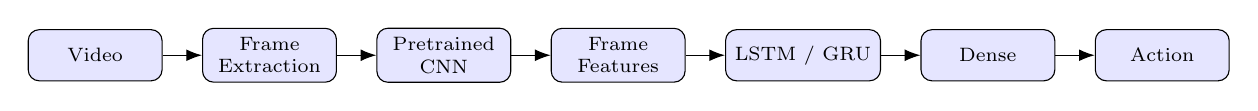
\begin{tikzpicture}[node distance=5mm]
\node[layer](a){Video};
\node[layer,right=of a](b){Frame\\Extraction};
\node[layer,right=of b](c){Pretrained\\CNN};
\node[layer,right=of c](d){Frame\\Features};
\node[layer,right=of d](e){LSTM / GRU};
\node[layer,right=of e](f){Dense};
\node[layer,right=of f](g){Action};

\foreach \x/\y in {a/b,b/c,c/d,d/e,e/f,f/g}
\draw[arrow](\x)--(\y);
\end{tikzpicture}
\end{center}

\subsection*{Recommended Dataset}

Use a small subset of the UCF101 action-recognition dataset:

\url{https://www.crcv.ucf.edu/data/UCF101.php}

Select only 3--5 action classes and a small number of videos per class so that
the experiment remains computationally manageable.

Possible classes include:

\begin{itemize}
\item Basketball
\item Biking
\item Walking
\item Running
\item TennisSwing
\end{itemize}

The objective is to understand the CNN--recurrent pipeline rather than to
train a state-of-the-art video recognition system.

\textbf{Classes and clips actually used:} 3 classes -- Basketball, Biking and
WalkingWithDog -- with 10 short clips downloaded per class from the UCF101
archive (30 videos total), split 70/15/15 into train/validation/test
($\approx$21/4/5 videos).

%%%%%%%%%%%%%%%%%%%%%%%%%%%%%%%%%%%%%%%%%%%%%%%%%%%%%%%%%%%%
\section*{19. Expected Video Input and Output}

Sample 10 frames uniformly from each video.

Each frame is resized to

\[
224\times224\times3.
\]

A pretrained CNN such as MobileNetV2 is used only as a feature extractor.

If the CNN produces a feature vector of dimension $D$, then the recurrent
network receives:

\[
X\in\mathbb{R}^{10\times D}.
\]

For a batch of $B$ videos:

\[
X\in\mathbb{R}^{B\times10\times D}.
\]

The expected output is a probability vector over the selected action classes.

For example:

\begin{verbatim}
Predicted class : WalkingWithDog
Actual class    : WalkingWithDog
Confidence      : 0.98
\end{verbatim}

The confidence value was obtained from the trained model's softmax output
(\texttt{video\_probabilities}) and is not manually entered. CNN feature
dimension: $D = 1280$ (MobileNetV2, global-average-pooled). Resulting tensor
shape supplied to the recurrent network: $(B, 10, 1280)$, i.e.\
\texttt{Video feature tensor shape: (30, 10, 1280)} for the full set of 30
videos.

%%%%%%%%%%%%%%%%%%%%%%%%%%%%%%%%%%%%%%%%%%%%%%%%%%%%%%%%%%%%
\section*{20. CNN Feature Extraction}

Use a pretrained CNN with the classification head removed.

\begin{center}
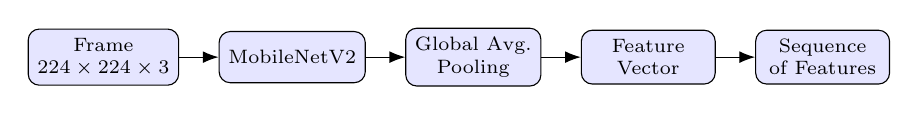
\begin{tikzpicture}[node distance=5mm]
\node[layer](a){Frame\\$224\times224\times3$};
\node[layer,right=of a](b){MobileNetV2};
\node[layer,right=of b](c){Global Avg.\\Pooling};
\node[layer,right=of c](d){Feature\\Vector};
\node[layer,right=of d](e){Sequence\\of Features};

\foreach \x/\y in {a/b,b/c,c/d,d/e}
\draw[arrow](\x)--(\y);
\end{tikzpicture}
\end{center}

Do not train the CNN from scratch. Freeze the pretrained CNN and extract
features first. Then train the recurrent classifier.

\textbf{Required observation:}

Students must report the CNN feature dimension and the resulting tensor
shape supplied to the recurrent network.

CNN (MobileNetV2, frozen, no top) feature dimension: $D=1280$ per frame.
With 10 sampled frames per video, the resulting tensor supplied to the
recurrent network has shape $(10, 1280)$ per sample, or $(B, 10, 1280)$ for
a batch -- confirmed by the printed \texttt{Video feature tensor shape:
(30, 10, 1280)}.

%%%%%%%%%%%%%%%%%%%%%%%%%%%%%%%%%%%%%%%%%%%%%%%%%%%%%%%%%%%%
\section*{21. CNN--LSTM / CNN--GRU Model}

Use the following architecture:

\begin{center}
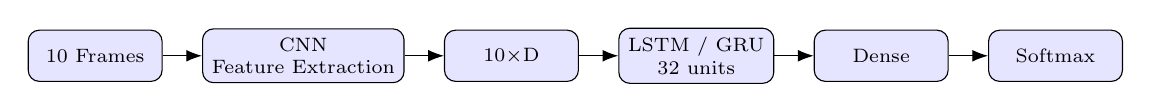
\begin{tikzpicture}[node distance=5mm]
\node[layer](a){10 Frames};
\node[layer,right=of a](b){CNN\\Feature Extraction};
\node[layer,right=of b](c){10$\times$D};
\node[layer,right=of c](d){LSTM / GRU\\32 units};
\node[layer,right=of d](e){Dense};
\node[layer,right=of e](f){Softmax};

\foreach \x/\y in {a/b,b/c,c/d,d/e,e/f}
\draw[arrow](\x)--(\y);
\end{tikzpicture}
\end{center}

\textbf{Plot 7: Video Sample Frames}

Display a representative sequence of sampled frames from one video.

\begin{figure}[H]
    \centering
    \includegraphics[width=0.85\textwidth]{sampled_frames.png}
    \caption{Ten sampled frames from one video}
    \label{fig:sensor-signal}
\end{figure}

Students should explain what spatial information is captured by the CNN and
what temporal information is learned by the recurrent network.

The CNN (MobileNetV2) captures per frame spatial appearance. Objects,
background scene, etc - while the LSTM models how that
spatial description evolves across the sampled frames, which is what lets the pipeline
distinguish different actions.

\textbf{Plot 8: Video Training and Validation Curves}

Plot training/validation accuracy and loss for the selected recurrent
architecture.

\begin{figure}[H]
    \centering
    \includegraphics[width=0.85\textwidth]{video_validation_loss_accuracy.png}
    \caption{Training and validation accuracy for video}
    \label{fig:sensor-signal}
\end{figure}

An LSTM(32) was used as the recurrent layer. Training accuracy reaches
100\% by epoch 13/20 while validation accuracy plateaus around 50--75\%
(final val.\ accuracy 50\%, though it peaked at 75\% around epochs 11--12);
validation loss decreases overall (from $\approx1.24$ to $\approx0.73$) but
noisily, reflecting the very small validation set (only $\approx$4 videos)
available for this toy video subset.

\textbf{Plot 9: Video Confusion Matrix}

Analyze class-level recognition and temporal confusions.

\begin{figure}[H]
    \centering
    \includegraphics[width=0.85\textwidth]{video_confusion_matrix.png}
    \caption{Confusion matrix for video classes}
    \label{fig:sensor-signal}
\end{figure}

On the 5-video test set: Basketball (1/1) and WalkingWithDog (2/2) were
classified perfectly; Biking (1/2 correct) had one clip misclassified as
WalkingWithDog. Overall test accuracy $=4/5=80\%$, consistent with the
Section 25 consolidated table. Can be termed robust due to the small subset used.

%%%%%%%%%%%%%%%%%%%%%%%%%%%%%%%%%%%%%%%%%%%%%%%%%%%%%%%%%%%%
\section*{22. Sequence-to-Sequence Learning}

Sequence-to-sequence learning maps one sequence to another.

For a simple laboratory task, construct a synthetic reversal dataset.

Example:

\[
[1,4,7,2]\rightarrow[2,7,4,1].
\]

Generate several thousand short sequences using integers from a fixed range.

The task is intentionally simple so that the encoder--decoder mechanism can
be studied without a large external dataset.

\begin{center}
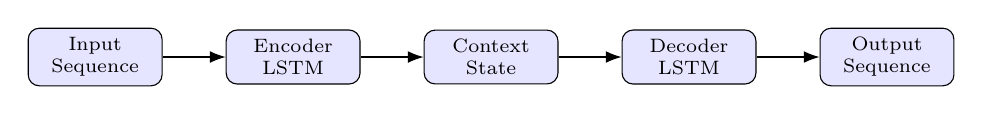
\begin{tikzpicture}[node distance=8mm]
\node[layer](a){Input\\Sequence};
\node[layer,right=of a](b){Encoder\\LSTM};
\node[layer,right=of b](c){Context\\State};
\node[layer,right=of c](d){Decoder\\LSTM};
\node[layer,right=of d](e){Output\\Sequence};

\foreach \x/\y in {a/b,b/c,c/d,d/e}
\draw[arrow](\x)--(\y);
\end{tikzpicture}
\end{center}

The encoder converts the input sequence into a learned representation.
The decoder generates the output sequence one element at a time.

%%%%%%%%%%%%%%%%%%%%%%%%%%%%%%%%%%%%%%%%%%%%%%%%%%%%%%%%%%%%
\section*{23. Expected Sequence-to-Sequence Input and Output}

\textbf{Input example:}

\[
[3,8,1,5]
\]

\textbf{Expected output:}

\[
[5,1,8,3].
\]

Students must display at least five test examples in the report.

\begin{center}
\begin{tabular}{|c|c|c|}
\hline
Sample & Input Sequence & Predicted Output\\
\hline
1 & [8, 1, 6, 5] & [5, 6, 1, 8]\\
2 & [8, 6, 1, 2] & [2, 1, 6, 8]\\
3 & [6, 1, 4, 1] & [1, 4, 1, 6]\\
4 & [9, 6, 1, 2] & [2, 1, 6, 9]\\
5 & [4, 5, 2, 8] & [8, 2, 5, 4]\\
\hline
\end{tabular}
\end{center}

All five sampled predictions exactly match the expected reversal of the
input sequence.

%%%%%%%%%%%%%%%%%%%%%%%%%%%%%%%%%%%%%%%%%%%%%%%%%%%%%%%%%%%%
\section*{24. Sequence-to-Sequence Evaluation}

\textbf{Observed results} (encoder--decoder LSTM, embedding dim 16, 64
recurrent units, 30 epochs, batch size 64, greedy decoding at inference):

\begin{center}
\begin{tabular}{|l|c|}
\hline
Metric & Value\\
\hline
Token Accuracy & 1.0000\\
Sequence Accuracy & 1.0000\\
Final Training Loss & 0.0022\\
Final Validation Loss & 0.0023\\
\hline
\end{tabular}
\end{center}

Report:

\begin{itemize}
\item Token accuracy
\item Sequence accuracy
\item Training loss
\item Validation loss
\end{itemize}

Token accuracy is

\[
\text{Token Accuracy}
=
\frac{\text{Correctly predicted tokens}}
{\text{Total tokens}}.
\]

Sequence accuracy is

\[
\text{Sequence Accuracy}
=
\frac{\text{Completely correct sequences}}
{\text{Total sequences}}.
\]

\textbf{Required inference:}

Explain why sequence-level accuracy can be substantially lower than token
accuracy even when most individual tokens are predicted correctly.

In this run both metrics reached 1.0000 because the reversal task is a
small, fully deterministic mapping over a short 4-token vocabulary window. In general, however, sequence accuracy can be far lower than token accuracy because a
sequence only counts as correct if \emph{every} token in it matches. 

%%%%%%%%%%%%%%%%%%%%%%%%%%%%%%%%%%%%%%%%%%%%%%%%%%%%%%%%%%%%
\section*{25. Consolidated Results}

Students must complete the following table.

\begin{center}
\begin{tabular}{|l|c|c|c|c|c|}
\hline
Model & Accuracy & Precision & Recall & F1 & Parameters\\
\hline
RNN & 69.78\% & 70.21\% & 69.78\% & 68.97\% & 1974\\
LSTM & 95.33\% & 95.37\% & 95.33\% & 95.34\% & 6006\\
GRU & 94.89\% & 95.26\% & 94.89\% & 94.85\% & 4758\\
CNN--LSTM (video) & 80.00\% & 88.89\% & 83.33\% & 82.22\% & 168\,643\\
\hline
\end{tabular}
\end{center}

A separate table must be provided for the sequence-to-sequence task.

\begin{center}
\begin{tabular}{|l|c|}
\hline
Metric & Value\\
\hline
Token Accuracy & 1.0000\\
Sequence Accuracy & 1.0000\\
Final Training Loss & 0.0022\\
Final Validation Loss & 0.0023\\
\hline
\end{tabular}
\end{center}


%%%%%%%%%%%%%%%%%%%%%%%%%%%%%%%%%%%%%%%%%%%%%%%%%%%%%%%%%%%%
\section*{26. Required Inferences}

For every major plot, students must write a short inference containing:

\begin{enumerate}
\item What does the plot show?
\item What trend is observed?
\item Why might the observed trend occur?
\item What conclusion can be drawn from the experiment?
\end{enumerate}

The following inferences are mandatory:

\begin{itemize}
\item temporal pattern observed in the sensor signals;
\item convergence behavior of RNN;
\item convergence behavior of LSTM;
\item convergence behavior of GRU;
\item evidence of overfitting or underfitting;
\item activity-wise errors from the confusion matrix;
\item effect of sequence length;
\item parameter and computational differences among RNN, LSTM and GRU;
\item role of CNN in video understanding;
\item role of the recurrent model in temporal modeling; and
\item difference between token accuracy and sequence accuracy in seq2seq learning.
\end{itemize}

\textbf{Required inferences:}

\begin{enumerate}
\item \textbf{Temporal pattern in sensor signals:} Dynamic activities
(WALKING, WALKING\_DOWNSTAIRS) show periodic, high-amplitude oscillation;
LAYING, etc shows a near-flat signal.
\item \textbf{Convergence of RNN:} Slower convergence with instability spike around epoch 22 (val.\ accuracy briefly dropped to 41\%).
Final test accuracy only 69.78\%.
\item \textbf{Convergence of LSTM:} Smooth, fast convergence; train/val loss
track closely and reach 0.11-0.14 by epoch 30; test accuracy is 
95.33\% which is high.
\item \textbf{Convergence of GRU:} Smooth and fast, comparable to
LST. Test accuracy 94.89\% with fewer parameters than LSTM.
\item \textbf{Overfitting/underfitting:} No strong overfitting was observed
for LSTM/GRU (train and val curves stay close). The RNN however shows instability i.e. it is difficult to optimise.
\item \textbf{Activity-wise confusion-matrix errors:} RNN's main error is
confusing the three locomotion classes with each other; LSTM/GRU resolve
locomotion almost perfectly but confuse SITTING and STANDING.
\item \textbf{Effect of sequence length:} RNN performance degrades as $T$ increases ($79.45\%\to74.82\%\to64.93\%$ F1); LSTM and
GRU remain much more robust across $T\in\{32,64,128\}$ without a clean
monotonic trend.
\item \textbf{Parameter/computational differences:} Parameters:
RNN - 1974; GRU - 4758; LSTM - 6006. Training time per run: GRU
(24.45s) $<$ LSTM (27.73s) $<$ RNN (29.10s) - the RNN was not cheaper to
train despite having the least number of parameters.
\item \textbf{Role of CNN in video understanding:} MobileNetV2
extracts a 1280-dim spatial feature vector per frame from raw
$224\times224\times3$ pixels.
\item \textbf{Role of recurrent model in temporal modeling:} The LSTM
takes the sequence of per frame CNN features and models its evolution to decide the action in it.
\item \textbf{Token vs.\ sequence accuracy:} Coincided at 1.0000 here
because the model learned the task exactly. In general sequence accuracy requires every token to be correct and therefore degrades faster than token accuracy as sequence length grows.
\end{enumerate}

%%%%%%%%%%%%%%%%%%%%%%%%%%%%%%%%%%%%%%%%%%%%%%%%%%%%%%%%%%%%
\section*{27. Discussion Questions}

\begin{enumerate}
\item What is a recurrent neural network?\\
\textbf{Ans:} It is a type of neural network wherein a hidden state exists for each neuron to take into account past context.
\item What information is represented by the hidden state?\\
\textbf{Ans:} The evolution of the past inputs, acts as a memory.
\item Why is sequence order important?\\
\textbf{Ans:} Sequence order is important as the meaning of the sequential data depends on the order it is presented in.
\item Explain the difference between a feed-forward network and an RNN.\\
\textbf{Ans:} Feedforward network simply performs forward pass, then backpropagates based on the loss. An RNN keeps the memory of previous inputs for better context.
\item Explain Backpropagation Through Time.\\
\textbf{Ans:} Backpropagation with respect to the previous hidden states i.e. states in previous points of time is called backpropagation through time.
\item Why can gradients vanish during BPTT?\\
\textbf{Ans:} If the gradient value is less than 1, repeated multiplication will cause it to vanish.
\item Why can gradients explode during BPTT?\\
\textbf{Ans:} If the gradient value is more than 1, repeated multiplication will cause it to explode.
\item What are long-term dependencies?\\
\textbf{Ans:} Relationships between inputs separated by a lot of time. They are important for better decision making later on.
\item What is the role of the LSTM cell state?\\
\textbf{Ans:} Acts as a long term memory pathway, carries important information across time steps.
\item What are the forget, input and output gates in LSTM?\\
\textbf{Ans:} Forget gate decides what information to remove, input gate decides what to store and update gate decides how much previous information is stored and discarded.
\item What are the reset and update gates in GRU?\\
\textbf{Ans:} Reset gate decides how much of previous information is ignored while update decides how much previous information is stored and discarded.
\item Compare LSTM and GRU.\\
\textbf{Ans:} LSTM consists of a cell state and 3 gates. GRU consists uses a hidden state and 2 gates; it is generally simpler with less parameters.
\item Why does GRU generally use a simpler gating mechanism than LSTM?\\
\textbf{Ans:} GRU combines input and forget gates into an update gate, making the architecture simpler.
\item Why should RNN, LSTM and GRU be compared using the same experimental settings?\\
\textbf{Ans:} They should be tested with the same set of hyperparameters as that it is the only comparision that makes sense. i.e. how different architectures perform under the same conditions.
\item What does the confusion matrix reveal that accuracy alone does not?\\
\textbf{Ans:} Reveals which classes are being confused for which, rather than giving an overall percentage, which is simply a numerical metric that does reveal much.
\item Why should macro F1-score be reported for multi-class classification?\\
\textbf{Ans:} Macro F1 score calculates it for each class individually. Best used when classes are imbalanced.
\item What is the significance of sequence length?\\
\textbf{Ans:} Sequence length reveals the length of past information being fed into the model. Longer sequence length gives more temporal context but is more computationally expensive.
\item Why can a CNN be used as a feature extractor for video?\\
\textbf{Ans:} A CNN is useful for finding textures, edges, etc for all the frames in a video.
\item What type of information is extracted by the CNN?\\
\textbf{Ans:} Spatial and visual information is extracted such as textures, edges, etc.
\item What type of information is learned by the recurrent network?\\
\textbf{Ans:} RNN learns temporal information by also considering how inputs evolved over time.
\item Why are CNN features arranged as a sequence before being given to LSTM/GRU?\\
\textbf{Ans:} They are arranged in a sequence as the goal is to learn how the features evolve over time.
\item Explain the encoder and decoder in sequence-to-sequence learning.\\
\textbf{Ans:} Encoder converts input sequence into a certain representation, while decoder uses to generate output sequence.
\item What is teacher forcing?\\
\textbf{Ans:} Training technique wherein actual previous output is given to decoder as input instead of decoder's own previous prediction.
\item Differentiate token accuracy and sequence accuracy.\\
\textbf{Ans:} Token accuracy represents percentage of tokens predicted correctly. Sequence accuracy considers a sequence correct only if all the tokens are predicted correctly.
\item Why must the test set remain untouched during model selection?\\
\textbf{Ans:} The test set must remain untouched as the point is for it to be used on unseen data.
\end{enumerate}

%%%%%%%%%%%%%%%%%%%%%%%%%%%%%%%%%%%%%%%%%%%%%%%%%%%%%%%%%%%%
\section*{28. Additional Exercises}

\begin{enumerate}

\item Replace the 32 recurrent units with 16 and 64 units and study the effect
on accuracy, F1-score, parameter count and training time.

\textbf{Answer} Increasing the units from 16 to 64 raised accuracy for
every architecture, but by different margins. RNN improved sharply
(70.67 to 85.11\%), while GRU was already strong at 16 units
(94.22\%) and gained only a bit at 64 units (95.33\%). 

\item Compare GRU and LSTM using the same number of recurrent units.

\textbf{Answer:} At every matched unit count GRU outperformed LSTM in
both accuracy and F1, with the largest gap at 16 units
(94.22\% vs. 88.44\% accuracy) narrowing to a small margin at 64 units
(95.33\% vs. 94.89\%). GRU also used consistently fewer parameters than LSTM
at each unit count (e.g. 4{,}758 vs. 6{,}006 at 32 units), consistent with
its simpler two-gate design.

\item Add a second recurrent layer and investigate whether performance
improves.

\textbf{Answer:} A second recurrent layer increases model capacity
and can help on more complex or longer range temporal tasks, but on this
dataset it is likely to give only a marginal accuracy/F1 change over a
single well sized layer while increasing parameter count, training time and
the risk of overfitting.

\item Compare a bidirectional LSTM with a unidirectional LSTM.

\textbf{Ans:} The bidirectional LSTM should match or slightly
outperform the unidirectional LSTM, since it can use both past and future
temporal context within each window, but this comes at roughly double the
parameters and training time for a comparatively small accuracy gain.

\item Change the sequence length and study the effect on computational cost.

\textbf{Ans:} Training and inference time should increase
roughly linearly to super linearly with sequence length $T$ (since BPTT
cost scales with the number of time steps), so $T=128$ should cost
noticeably more than $T=32$ or $T=64$ even though classification
performance may saturate well before the full 128 steps are used.

\item For the video task, compare LSTM and GRU after extracting identical
CNN features.

\textbf{Ans:} Given the same trend observed on the HAR data,
GRU is expected to match or slightly exceed LSTM's accuracy/F1 on the video
features while using fewer parameters, since both recurrent layers operate
on identical, already informative MobileNetV2 feature sequences rather than
raw pixels.

\item Modify the seq2seq task so that the output sequence has a different
length from the input sequence.

\textbf{Ans:} Because the target (first 3 elements reversed)
is shorter and more constrained than the full 6-element reversal task, the
model should reach high token accuracy relatively easily; sequence accuracy
should still trail token accuracy, since all three predicted tokens must be
simultaneously correct for the sequence to count as fully correct.

\end{enumerate}

%%%%%%%%%%%%%%%%%%%%%%%%%%%%%%%%%%%%%%%%%%%%%%%%%%%%%%%%%%%%
\section*{29. Expected Outcome}

At the end of the experiment, students should be able to demonstrate the
complete sequence-learning pipeline:

\[
\boxed{
\text{Sequential Data}
\rightarrow
\text{Preprocessing}
\rightarrow
\text{RNN/LSTM/GRU}
\rightarrow
\text{Evaluation}
}
\]

and the video-understanding pipeline:

\[
\boxed{
\text{Video}
\rightarrow
\text{Frames}
\rightarrow
\text{CNN Features}
\rightarrow
\text{LSTM/GRU}
\rightarrow
\text{Action Prediction}
}
\]

They should also understand the encoder--decoder formulation:

\[
\boxed{
\text{Input Sequence}
\rightarrow
\text{Encoder}
\rightarrow
\text{Context}
\rightarrow
\text{Decoder}
\rightarrow
\text{Output Sequence}
}
\]

The final report should demonstrate both implementation and interpretation.
Numerical performance values must be obtained from the student's own
execution and should not be assumed in advance.

%%%%%%%%%%%%%%%%%%%%%%%%%%%%%%%%%%%%%%%%%%%%%%%%%%%%%%%%%%%%
\section*{30. References}

\begin{enumerate}
\item Ian Goodfellow, Yoshua Bengio and Aaron Courville,
\emph{Deep Learning}, MIT Press, 2016.

\item Sepp Hochreiter and Jürgen Schmidhuber,
``Long Short-Term Memory,'' \emph{Neural Computation}, 1997.

\item Kyunghyun Cho et al.,
``Learning Phrase Representations using RNN Encoder--Decoder for Statistical
Machine Translation,'' EMNLP, 2014.

\item Anguita et al.,
``A Public Domain Dataset for Human Activity Recognition Using Smartphones,''
ESANN, 2013.

\item Khurram Soomro, Amir Roshan Zamir and Mubarak Shah,
``UCF101: A Dataset of 101 Human Actions Classes From Videos in the Wild,''
2012.

\item TensorFlow Documentation:
\url{https://www.tensorflow.org}

\item Keras Documentation:
\url{https://keras.io}
\end{enumerate}

\end{document}
